\documentclass[twoside]{book}

% Packages required by doxygen
\usepackage{fixltx2e}
\usepackage{calc}
\usepackage{doxygen}
\usepackage[export]{adjustbox} % also loads graphicx
\usepackage{graphicx}
\usepackage[utf8]{inputenc}
\usepackage{makeidx}
\usepackage{multicol}
\usepackage{multirow}
\PassOptionsToPackage{warn}{textcomp}
\usepackage{textcomp}
\usepackage[nointegrals]{wasysym}
\usepackage[table]{xcolor}

% Font selection
\usepackage[T1]{fontenc}
\usepackage[scaled=.90]{helvet}
\usepackage{courier}
\usepackage{amssymb}
\usepackage{sectsty}
\renewcommand{\familydefault}{\sfdefault}
\allsectionsfont{%
  \fontseries{bc}\selectfont%
  \color{darkgray}%
}
\renewcommand{\DoxyLabelFont}{%
  \fontseries{bc}\selectfont%
  \color{darkgray}%
}
\newcommand{\+}{\discretionary{\mbox{\scriptsize$\hookleftarrow$}}{}{}}

% Page & text layout
\usepackage{geometry}
\geometry{%
  a4paper,%
  top=2.5cm,%
  bottom=2.5cm,%
  left=2.5cm,%
  right=2.5cm%
}
\tolerance=750
\hfuzz=15pt
\hbadness=750
\setlength{\emergencystretch}{15pt}
\setlength{\parindent}{0cm}
\setlength{\parskip}{3ex plus 2ex minus 2ex}
\makeatletter
\renewcommand{\paragraph}{%
  \@startsection{paragraph}{4}{0ex}{-1.0ex}{1.0ex}{%
    \normalfont\normalsize\bfseries\SS@parafont%
  }%
}
\renewcommand{\subparagraph}{%
  \@startsection{subparagraph}{5}{0ex}{-1.0ex}{1.0ex}{%
    \normalfont\normalsize\bfseries\SS@subparafont%
  }%
}
\makeatother

% Headers & footers
\usepackage{fancyhdr}
\pagestyle{fancyplain}
\fancyhead[LE]{\fancyplain{}{\bfseries\thepage}}
\fancyhead[CE]{\fancyplain{}{}}
\fancyhead[RE]{\fancyplain{}{\bfseries\leftmark}}
\fancyhead[LO]{\fancyplain{}{\bfseries\rightmark}}
\fancyhead[CO]{\fancyplain{}{}}
\fancyhead[RO]{\fancyplain{}{\bfseries\thepage}}
\fancyfoot[LE]{\fancyplain{}{}}
\fancyfoot[CE]{\fancyplain{}{}}
\fancyfoot[RE]{\fancyplain{}{\bfseries\scriptsize Generated by Doxygen }}
\fancyfoot[LO]{\fancyplain{}{\bfseries\scriptsize Generated by Doxygen }}
\fancyfoot[CO]{\fancyplain{}{}}
\fancyfoot[RO]{\fancyplain{}{}}
\renewcommand{\footrulewidth}{0.4pt}
\renewcommand{\chaptermark}[1]{%
  \markboth{#1}{}%
}
\renewcommand{\sectionmark}[1]{%
  \markright{\thesection\ #1}%
}

% Indices & bibliography
\usepackage{natbib}
\usepackage[titles]{tocloft}
\setcounter{tocdepth}{3}
\setcounter{secnumdepth}{5}
\makeindex

% Hyperlinks (required, but should be loaded last)
\usepackage{ifpdf}
\ifpdf
  \usepackage[pdftex,pagebackref=true]{hyperref}
\else
  \usepackage[ps2pdf,pagebackref=true]{hyperref}
\fi
\hypersetup{%
  colorlinks=true,%
  linkcolor=blue,%
  citecolor=blue,%
  unicode%
}

% Custom commands
\newcommand{\clearemptydoublepage}{%
  \newpage{\pagestyle{empty}\cleardoublepage}%
}

\usepackage{caption}
\captionsetup{labelsep=space,justification=centering,font={bf},singlelinecheck=off,skip=4pt,position=top}

%===== C O N T E N T S =====

\begin{document}

% Titlepage & ToC
\hypersetup{pageanchor=false,
             bookmarksnumbered=true,
             pdfencoding=unicode
            }
\pagenumbering{alph}
\begin{titlepage}
\vspace*{7cm}
\begin{center}%
{\Large Merger }\\
\vspace*{1cm}
{\large Generated by Doxygen 1.8.13}\\
\end{center}
\end{titlepage}
\clearemptydoublepage
\pagenumbering{roman}
\tableofcontents
\clearemptydoublepage
\pagenumbering{arabic}
\hypersetup{pageanchor=true}

%--- Begin generated contents ---
\chapter{Hierarchical Index}
\section{Class Hierarchy}
This inheritance list is sorted roughly, but not completely, alphabetically\+:\begin{DoxyCompactList}
\item \contentsline{section}{Column\+Vector}{\pageref{classColumnVector}}{}
\item \contentsline{section}{Matrix}{\pageref{classMatrix}}{}
\item \contentsline{section}{Model\+Factory}{\pageref{classModelFactory}}{}
\item \contentsline{section}{Model\+Interface}{\pageref{classModelInterface}}{}
\begin{DoxyCompactList}
\item \contentsline{section}{Linear\+Demands\+Constant\+Costs}{\pageref{classLinearDemandsConstantCosts}}{}
\end{DoxyCompactList}
\item Q\+Abstract\+Table\+Model\begin{DoxyCompactList}
\item \contentsline{section}{Model\+Table\+Data}{\pageref{classModelTableData}}{}
\end{DoxyCompactList}
\item Q\+Main\+Window\begin{DoxyCompactList}
\item \contentsline{section}{Main\+Window}{\pageref{classMainWindow}}{}
\item \contentsline{section}{Model\+Window}{\pageref{classModelWindow}}{}
\end{DoxyCompactList}
\item Q\+Table\+View\begin{DoxyCompactList}
\item \contentsline{section}{Model\+Table\+View}{\pageref{classModelTableView}}{}
\end{DoxyCompactList}
\item Q\+Widget\begin{DoxyCompactList}
\item \contentsline{section}{Load\+Model\+Widget}{\pageref{classLoadModelWidget}}{}
\end{DoxyCompactList}
\item \contentsline{section}{Row\+Vector}{\pageref{classRowVector}}{}
\end{DoxyCompactList}

\chapter{Class Index}
\section{Class List}
Here are the classes, structs, unions and interfaces with brief descriptions\+:\begin{DoxyCompactList}
\item\contentsline{section}{\hyperlink{classColumnVector}{Column\+Vector} }{\pageref{classColumnVector}}{}
\item\contentsline{section}{\hyperlink{classLinearDemandsConstantCosts}{Linear\+Demands\+Constant\+Costs} \\*Model in which demands follow a linear function and costs are constant }{\pageref{classLinearDemandsConstantCosts}}{}
\item\contentsline{section}{\hyperlink{classMainWindow}{Main\+Window} }{\pageref{classMainWindow}}{}
\item\contentsline{section}{\hyperlink{classMatrix}{Matrix} }{\pageref{classMatrix}}{}
\item\contentsline{section}{\hyperlink{classModelInterface}{Model\+Interface} \\*An interface for any model }{\pageref{classModelInterface}}{}
\item\contentsline{section}{\hyperlink{classModelResult}{Model\+Result} }{\pageref{classModelResult}}{}
\item\contentsline{section}{\hyperlink{classModelWidget}{Model\+Widget} }{\pageref{classModelWidget}}{}
\item\contentsline{section}{\hyperlink{classRowVector}{Row\+Vector} }{\pageref{classRowVector}}{}
\end{DoxyCompactList}

\chapter{Class Documentation}
\hypertarget{classColumnVector}{}\section{Column\+Vector Class Reference}
\label{classColumnVector}\index{Column\+Vector@{Column\+Vector}}
\subsection*{Public Member Functions}
\begin{DoxyCompactItemize}
\item 
\mbox{\Hypertarget{classColumnVector_a04c6fb8d73a6a1e816246114487af21e}\label{classColumnVector_a04c6fb8d73a6a1e816246114487af21e}} 
{\bfseries Column\+Vector} (int n)
\item 
\mbox{\Hypertarget{classColumnVector_ace00809de2f40bc40760759915424606}\label{classColumnVector_ace00809de2f40bc40760759915424606}} 
int {\bfseries Size} () const
\item 
\mbox{\Hypertarget{classColumnVector_a71aef8eb58f6abf7142aa064ea4b2b67}\label{classColumnVector_a71aef8eb58f6abf7142aa064ea4b2b67}} 
\hyperlink{classColumnVector}{Column\+Vector} {\bfseries operator+} (\hyperlink{classColumnVector}{Column\+Vector} const \&other) const
\item 
\mbox{\Hypertarget{classColumnVector_a9a97a16318637c348473c2ef010772e0}\label{classColumnVector_a9a97a16318637c348473c2ef010772e0}} 
\hyperlink{classColumnVector}{Column\+Vector} \& {\bfseries operator+=} (\hyperlink{classColumnVector}{Column\+Vector} const \&other)
\item 
\mbox{\Hypertarget{classColumnVector_a2955856b4cf0c90840e927192007b717}\label{classColumnVector_a2955856b4cf0c90840e927192007b717}} 
\hyperlink{classColumnVector}{Column\+Vector} {\bfseries operator-\/} (\hyperlink{classColumnVector}{Column\+Vector} const \&other) const
\item 
\mbox{\Hypertarget{classColumnVector_a2eabe166745011663d3f02454d04b526}\label{classColumnVector_a2eabe166745011663d3f02454d04b526}} 
\hyperlink{classColumnVector}{Column\+Vector} \& {\bfseries operator-\/=} (\hyperlink{classColumnVector}{Column\+Vector} const \&other)
\item 
\mbox{\Hypertarget{classColumnVector_a48b64ae9de4f9feff9712093d5baf3c4}\label{classColumnVector_a48b64ae9de4f9feff9712093d5baf3c4}} 
\hyperlink{classColumnVector}{Column\+Vector} {\bfseries operator$\ast$} (double other) const
\item 
\mbox{\Hypertarget{classColumnVector_a9cac6c2fb1c1adcc8aec577e9fa43981}\label{classColumnVector_a9cac6c2fb1c1adcc8aec577e9fa43981}} 
\hyperlink{classColumnVector}{Column\+Vector} \& {\bfseries operator$\ast$=} (double other)
\item 
\mbox{\Hypertarget{classColumnVector_a509eb2c7108dd1870f7282a3eb9038c1}\label{classColumnVector_a509eb2c7108dd1870f7282a3eb9038c1}} 
\hyperlink{classColumnVector}{Column\+Vector} {\bfseries operator\%} (\hyperlink{classColumnVector}{Column\+Vector} const \&other) const
\item 
\mbox{\Hypertarget{classColumnVector_afe72f924a5a097ad3386576c6fe950bf}\label{classColumnVector_afe72f924a5a097ad3386576c6fe950bf}} 
\hyperlink{classColumnVector}{Column\+Vector} \& {\bfseries operator\%=} (\hyperlink{classColumnVector}{Column\+Vector} const \&other)
\item 
\mbox{\Hypertarget{classColumnVector_a27f20757b2d702147f5b70a966e17b6c}\label{classColumnVector_a27f20757b2d702147f5b70a966e17b6c}} 
double \& {\bfseries operator\mbox{[}$\,$\mbox{]}} (int index)
\item 
\mbox{\Hypertarget{classColumnVector_a205d763788746d98810ec1d7541fc20f}\label{classColumnVector_a205d763788746d98810ec1d7541fc20f}} 
double const  \& {\bfseries operator\mbox{[}$\,$\mbox{]}} (int index) const
\end{DoxyCompactItemize}


\subsection{Detailed Description}


Definition at line 10 of file column\+\_\+vector.\+h.



The documentation for this class was generated from the following files\+:\begin{DoxyCompactItemize}
\item 
Utils/column\+\_\+vector.\+h\item 
Utils/column\+\_\+vector.\+cpp\end{DoxyCompactItemize}

\hypertarget{classFirmWidget}{}\section{Firm\+Widget Class Reference}
\label{classFirmWidget}\index{Firm\+Widget@{Firm\+Widget}}


Inheritance diagram for Firm\+Widget\+:
\nopagebreak
\begin{figure}[H]
\begin{center}
\leavevmode
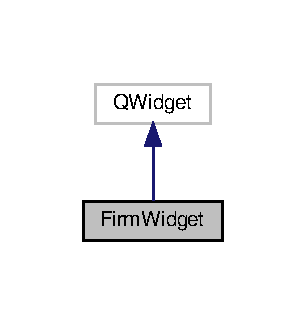
\includegraphics[width=147pt]{classFirmWidget__inherit__graph}
\end{center}
\end{figure}


Collaboration diagram for Firm\+Widget\+:
\nopagebreak
\begin{figure}[H]
\begin{center}
\leavevmode
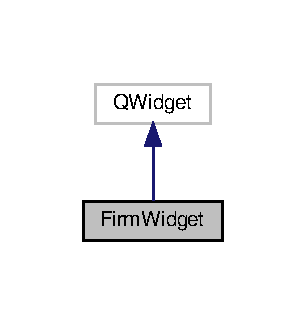
\includegraphics[width=147pt]{classFirmWidget__coll__graph}
\end{center}
\end{figure}
\subsection*{Public Member Functions}
\begin{DoxyCompactItemize}
\item 
\mbox{\Hypertarget{classFirmWidget_a67b0b5242477f5523a6e00874f4d8af5}\label{classFirmWidget_a67b0b5242477f5523a6e00874f4d8af5}} 
{\bfseries Firm\+Widget} (Q\+Widget $\ast$parent=nullptr)
\end{DoxyCompactItemize}


\subsection{Detailed Description}


Definition at line 8 of file firm\+\_\+widget.\+h.



The documentation for this class was generated from the following files\+:\begin{DoxyCompactItemize}
\item 
G\+U\+I/\+Model\+Window/\+Merge\+Dialog/\+Helpers/firm\+\_\+widget.\+h\item 
G\+U\+I/\+Model\+Window/\+Merge\+Dialog/\+Helpers/firm\+\_\+widget.\+cpp\end{DoxyCompactItemize}

\hypertarget{classLinearDemandsConstantCosts}{}\section{Linear\+Demands\+Constant\+Costs Class Reference}
\label{classLinearDemandsConstantCosts}\index{Linear\+Demands\+Constant\+Costs@{Linear\+Demands\+Constant\+Costs}}


A model in which demands follow a linear function and costs are constant.  




{\ttfamily \#include $<$linear\+\_\+demands\+\_\+constant\+\_\+costs.\+h$>$}



Inheritance diagram for Linear\+Demands\+Constant\+Costs\+:\nopagebreak
\begin{figure}[H]
\begin{center}
\leavevmode
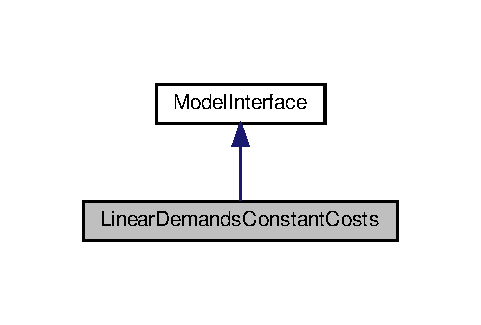
\includegraphics[width=231pt]{classLinearDemandsConstantCosts__inherit__graph}
\end{center}
\end{figure}


Collaboration diagram for Linear\+Demands\+Constant\+Costs\+:\nopagebreak
\begin{figure}[H]
\begin{center}
\leavevmode
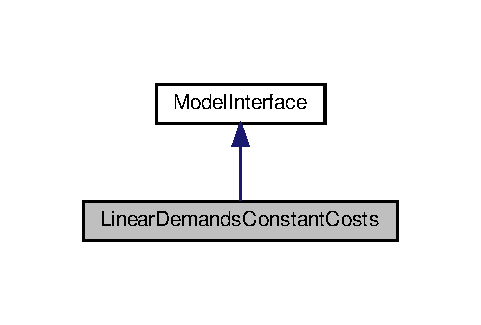
\includegraphics[width=231pt]{classLinearDemandsConstantCosts__coll__graph}
\end{center}
\end{figure}
\subsection*{Public Member Functions}
\begin{DoxyCompactItemize}
\item 
\hyperlink{classLinearDemandsConstantCosts_a79e3cc71f551a3ad3ecfd5ea3818a6c0}{Linear\+Demands\+Constant\+Costs} ()=default
\item 
\hyperlink{classLinearDemandsConstantCosts_a0a7e9c271148594fdc0e4024cfd521a9}{Linear\+Demands\+Constant\+Costs} (\hyperlink{classColumnVector}{Column\+Vector} const \&income, \hyperlink{classColumnVector}{Column\+Vector} const \&costs, \hyperlink{classMatrix}{Matrix} const \&elasticities)
\item 
\mbox{\Hypertarget{classLinearDemandsConstantCosts_a583af2ebff9e7d09ab02270c97ed57ba}\label{classLinearDemandsConstantCosts_a583af2ebff9e7d09ab02270c97ed57ba}} 
virtual Model\+Type \hyperlink{classLinearDemandsConstantCosts_a583af2ebff9e7d09ab02270c97ed57ba}{Get\+Type} () const override final
\begin{DoxyCompactList}\small\item\em Returns the type of the model. \end{DoxyCompactList}\item 
\mbox{\Hypertarget{classLinearDemandsConstantCosts_ad968f45ba4a6e9d36b96c1ab92980eb5}\label{classLinearDemandsConstantCosts_ad968f45ba4a6e9d36b96c1ab92980eb5}} 
virtual int \hyperlink{classLinearDemandsConstantCosts_ad968f45ba4a6e9d36b96c1ab92980eb5}{Get\+Number\+Of\+Products} () const override final
\begin{DoxyCompactList}\small\item\em Returns the number of products. \end{DoxyCompactList}\item 
\mbox{\Hypertarget{classLinearDemandsConstantCosts_ae2f4565860b89a5576b54884a4d520d1}\label{classLinearDemandsConstantCosts_ae2f4565860b89a5576b54884a4d520d1}} 
virtual \hyperlink{classColumnVector}{Column\+Vector} \hyperlink{classLinearDemandsConstantCosts_ae2f4565860b89a5576b54884a4d520d1}{Compute\+Prices} () const override final
\begin{DoxyCompactList}\small\item\em Computes the equilibrium prices of the model. \end{DoxyCompactList}\item 
virtual \hyperlink{classColumnVector}{Column\+Vector} \hyperlink{classLinearDemandsConstantCosts_a310864e458935098502561540a71a88c}{Compute\+Quantities} (\hyperlink{classColumnVector}{Column\+Vector} const \&prices) const override final
\item 
virtual \hyperlink{classColumnVector}{Column\+Vector} \hyperlink{classLinearDemandsConstantCosts_a74f907b4737865de086c8aa1f125d7c8}{Compute\+Costs} (\hyperlink{classColumnVector}{Column\+Vector} const \&quantities) const override final
\item 
virtual \hyperlink{classColumnVector}{Column\+Vector} \hyperlink{classLinearDemandsConstantCosts_a48b52dab01d2cf45beae51eab615f7ae}{Compute\+Profits} (\hyperlink{classColumnVector}{Column\+Vector} const \&prices) const override final
\item 
virtual \hyperlink{classColumnVector}{Column\+Vector} \hyperlink{classLinearDemandsConstantCosts_a9d3fa6a3b151c2f1703f23bbee6954cb}{Compute\+Consumer\+Welfare} (\hyperlink{classColumnVector}{Column\+Vector} const \&prices) const override final
\item 
virtual void \hyperlink{classLinearDemandsConstantCosts_a0ee422d927b5a85f9aba8782b02f537b}{Merge} (int i, int j) override final
\item 
virtual bool \hyperlink{classLinearDemandsConstantCosts_a91ba117b740d0e5cb5d6efd63d61a5f6}{Are\+Produced\+By\+Same\+Firm} (int i, int j) const override final
\item 
virtual void \hyperlink{classLinearDemandsConstantCosts_aef2823751866a4933a8611dd4622d78b}{Save\+To\+File} (std\+::string const \&file\+\_\+path) const override final
\item 
virtual void \hyperlink{classLinearDemandsConstantCosts_a075add461e368629b9dfd8f72033e2ad}{Load\+From\+File} (std\+::string const \&file\+\_\+path) override final
\end{DoxyCompactItemize}


\subsection{Detailed Description}
A model in which demands follow a linear function and costs are constant. 

A model in which the demands vector can be written as

\begin{equation} q = a + B' p \end{equation}

where $ a $ is the income vector, $ p $ is the vector of prices and $ B $ is the elasticities\textquotesingle{} matrix. Besides, it defines a $ c $ vector that is constant. 

Definition at line 17 of file linear\+\_\+demands\+\_\+constant\+\_\+costs.\+h.



\subsection{Constructor \& Destructor Documentation}
\mbox{\Hypertarget{classLinearDemandsConstantCosts_a79e3cc71f551a3ad3ecfd5ea3818a6c0}\label{classLinearDemandsConstantCosts_a79e3cc71f551a3ad3ecfd5ea3818a6c0}} 
\index{Linear\+Demands\+Constant\+Costs@{Linear\+Demands\+Constant\+Costs}!Linear\+Demands\+Constant\+Costs@{Linear\+Demands\+Constant\+Costs}}
\index{Linear\+Demands\+Constant\+Costs@{Linear\+Demands\+Constant\+Costs}!Linear\+Demands\+Constant\+Costs@{Linear\+Demands\+Constant\+Costs}}
\subsubsection{\texorpdfstring{Linear\+Demands\+Constant\+Costs()}{LinearDemandsConstantCosts()}\hspace{0.1cm}{\footnotesize\ttfamily [1/2]}}
{\footnotesize\ttfamily Linear\+Demands\+Constant\+Costs\+::\+Linear\+Demands\+Constant\+Costs (\begin{DoxyParamCaption}{ }\end{DoxyParamCaption})\hspace{0.3cm}{\ttfamily [default]}}

Creates a model with no products. It should only be used to load the model from a file after calling it. \mbox{\Hypertarget{classLinearDemandsConstantCosts_a0a7e9c271148594fdc0e4024cfd521a9}\label{classLinearDemandsConstantCosts_a0a7e9c271148594fdc0e4024cfd521a9}} 
\index{Linear\+Demands\+Constant\+Costs@{Linear\+Demands\+Constant\+Costs}!Linear\+Demands\+Constant\+Costs@{Linear\+Demands\+Constant\+Costs}}
\index{Linear\+Demands\+Constant\+Costs@{Linear\+Demands\+Constant\+Costs}!Linear\+Demands\+Constant\+Costs@{Linear\+Demands\+Constant\+Costs}}
\subsubsection{\texorpdfstring{Linear\+Demands\+Constant\+Costs()}{LinearDemandsConstantCosts()}\hspace{0.1cm}{\footnotesize\ttfamily [2/2]}}
{\footnotesize\ttfamily Linear\+Demands\+Constant\+Costs\+::\+Linear\+Demands\+Constant\+Costs (\begin{DoxyParamCaption}\item[{\hyperlink{classColumnVector}{Column\+Vector} const \&}]{income,  }\item[{\hyperlink{classColumnVector}{Column\+Vector} const \&}]{costs,  }\item[{\hyperlink{classMatrix}{Matrix} const \&}]{elasticities }\end{DoxyParamCaption})}

Creates a model with {\ttfamily income} being $ a $, {\ttfamily costs} being $ c $ and {\ttfamily elasticities} being $ B $ in the model definition.


\begin{DoxyParams}{Parameters}
{\em income} & The income vector as defined in the model. \\
\hline
{\em costs} & The costs vector as defined in the model. \\
\hline
{\em elasticities} & The matrix of elasticities as defined in the model. \\
\hline
\end{DoxyParams}


Definition at line 5 of file linear\+\_\+demands\+\_\+constant\+\_\+costs.\+cpp.



\subsection{Member Function Documentation}
\mbox{\Hypertarget{classLinearDemandsConstantCosts_a91ba117b740d0e5cb5d6efd63d61a5f6}\label{classLinearDemandsConstantCosts_a91ba117b740d0e5cb5d6efd63d61a5f6}} 
\index{Linear\+Demands\+Constant\+Costs@{Linear\+Demands\+Constant\+Costs}!Are\+Produced\+By\+Same\+Firm@{Are\+Produced\+By\+Same\+Firm}}
\index{Are\+Produced\+By\+Same\+Firm@{Are\+Produced\+By\+Same\+Firm}!Linear\+Demands\+Constant\+Costs@{Linear\+Demands\+Constant\+Costs}}
\subsubsection{\texorpdfstring{Are\+Produced\+By\+Same\+Firm()}{AreProducedBySameFirm()}}
{\footnotesize\ttfamily bool Linear\+Demands\+Constant\+Costs\+::\+Are\+Produced\+By\+Same\+Firm (\begin{DoxyParamCaption}\item[{int}]{i,  }\item[{int}]{j }\end{DoxyParamCaption}) const\hspace{0.3cm}{\ttfamily [final]}, {\ttfamily [override]}, {\ttfamily [virtual]}}

Returns true iff the two given products are produced by the same firm.


\begin{DoxyParams}{Parameters}
{\em i} & The index of the first product. \\
\hline
{\em j} & The index of the second product. \\
\hline
\end{DoxyParams}


Implements \hyperlink{classModelInterface_abbc3c44c6d41b596b6201a9e61e1ff83}{Model\+Interface}.



Definition at line 50 of file linear\+\_\+demands\+\_\+constant\+\_\+costs.\+cpp.

\mbox{\Hypertarget{classLinearDemandsConstantCosts_a9d3fa6a3b151c2f1703f23bbee6954cb}\label{classLinearDemandsConstantCosts_a9d3fa6a3b151c2f1703f23bbee6954cb}} 
\index{Linear\+Demands\+Constant\+Costs@{Linear\+Demands\+Constant\+Costs}!Compute\+Consumer\+Welfare@{Compute\+Consumer\+Welfare}}
\index{Compute\+Consumer\+Welfare@{Compute\+Consumer\+Welfare}!Linear\+Demands\+Constant\+Costs@{Linear\+Demands\+Constant\+Costs}}
\subsubsection{\texorpdfstring{Compute\+Consumer\+Welfare()}{ComputeConsumerWelfare()}}
{\footnotesize\ttfamily \hyperlink{classColumnVector}{Column\+Vector} Linear\+Demands\+Constant\+Costs\+::\+Compute\+Consumer\+Welfare (\begin{DoxyParamCaption}\item[{\hyperlink{classColumnVector}{Column\+Vector} const \&}]{prices }\end{DoxyParamCaption}) const\hspace{0.3cm}{\ttfamily [final]}, {\ttfamily [override]}, {\ttfamily [virtual]}}

Computes the consumer welfare of the model in equilibrium.


\begin{DoxyParams}{Parameters}
{\em prices} & The equilibrium prices. \\
\hline
\end{DoxyParams}


Implements \hyperlink{classModelInterface_a094ebb85618fb13bf38f6faff1f5dd7b}{Model\+Interface}.



Definition at line 35 of file linear\+\_\+demands\+\_\+constant\+\_\+costs.\+cpp.

\mbox{\Hypertarget{classLinearDemandsConstantCosts_a74f907b4737865de086c8aa1f125d7c8}\label{classLinearDemandsConstantCosts_a74f907b4737865de086c8aa1f125d7c8}} 
\index{Linear\+Demands\+Constant\+Costs@{Linear\+Demands\+Constant\+Costs}!Compute\+Costs@{Compute\+Costs}}
\index{Compute\+Costs@{Compute\+Costs}!Linear\+Demands\+Constant\+Costs@{Linear\+Demands\+Constant\+Costs}}
\subsubsection{\texorpdfstring{Compute\+Costs()}{ComputeCosts()}}
{\footnotesize\ttfamily virtual \hyperlink{classColumnVector}{Column\+Vector} Linear\+Demands\+Constant\+Costs\+::\+Compute\+Costs (\begin{DoxyParamCaption}\item[{\hyperlink{classColumnVector}{Column\+Vector} const \&}]{quantities }\end{DoxyParamCaption}) const\hspace{0.3cm}{\ttfamily [inline]}, {\ttfamily [final]}, {\ttfamily [override]}, {\ttfamily [virtual]}}

Computes the costs of the model in equilibrium.


\begin{DoxyParams}{Parameters}
{\em quantities} & The equilibrium quantities. \\
\hline
\end{DoxyParams}


Implements \hyperlink{classModelInterface_ac0a7cc3db9fc177dc75f16abf00275a7}{Model\+Interface}.



Definition at line 53 of file linear\+\_\+demands\+\_\+constant\+\_\+costs.\+h.

\mbox{\Hypertarget{classLinearDemandsConstantCosts_a48b52dab01d2cf45beae51eab615f7ae}\label{classLinearDemandsConstantCosts_a48b52dab01d2cf45beae51eab615f7ae}} 
\index{Linear\+Demands\+Constant\+Costs@{Linear\+Demands\+Constant\+Costs}!Compute\+Profits@{Compute\+Profits}}
\index{Compute\+Profits@{Compute\+Profits}!Linear\+Demands\+Constant\+Costs@{Linear\+Demands\+Constant\+Costs}}
\subsubsection{\texorpdfstring{Compute\+Profits()}{ComputeProfits()}}
{\footnotesize\ttfamily \hyperlink{classColumnVector}{Column\+Vector} Linear\+Demands\+Constant\+Costs\+::\+Compute\+Profits (\begin{DoxyParamCaption}\item[{\hyperlink{classColumnVector}{Column\+Vector} const \&}]{prices }\end{DoxyParamCaption}) const\hspace{0.3cm}{\ttfamily [final]}, {\ttfamily [override]}, {\ttfamily [virtual]}}

Computes the profits of the model in equilibrium.


\begin{DoxyParams}{Parameters}
{\em prices} & The equilibrium prices. \\
\hline
\end{DoxyParams}


Implements \hyperlink{classModelInterface_a311a000060cece8fc1058cd27bf07864}{Model\+Interface}.



Definition at line 30 of file linear\+\_\+demands\+\_\+constant\+\_\+costs.\+cpp.

\mbox{\Hypertarget{classLinearDemandsConstantCosts_a310864e458935098502561540a71a88c}\label{classLinearDemandsConstantCosts_a310864e458935098502561540a71a88c}} 
\index{Linear\+Demands\+Constant\+Costs@{Linear\+Demands\+Constant\+Costs}!Compute\+Quantities@{Compute\+Quantities}}
\index{Compute\+Quantities@{Compute\+Quantities}!Linear\+Demands\+Constant\+Costs@{Linear\+Demands\+Constant\+Costs}}
\subsubsection{\texorpdfstring{Compute\+Quantities()}{ComputeQuantities()}}
{\footnotesize\ttfamily \hyperlink{classColumnVector}{Column\+Vector} Linear\+Demands\+Constant\+Costs\+::\+Compute\+Quantities (\begin{DoxyParamCaption}\item[{\hyperlink{classColumnVector}{Column\+Vector} const \&}]{prices }\end{DoxyParamCaption}) const\hspace{0.3cm}{\ttfamily [final]}, {\ttfamily [override]}, {\ttfamily [virtual]}}

Computes the equilibrium quantities of the model.


\begin{DoxyParams}{Parameters}
{\em prices} & The equilibrium prices. \\
\hline
\end{DoxyParams}


Implements \hyperlink{classModelInterface_af9a936f6f0d1b1f0f2c5bf35785e7db4}{Model\+Interface}.



Definition at line 25 of file linear\+\_\+demands\+\_\+constant\+\_\+costs.\+cpp.

\mbox{\Hypertarget{classLinearDemandsConstantCosts_a075add461e368629b9dfd8f72033e2ad}\label{classLinearDemandsConstantCosts_a075add461e368629b9dfd8f72033e2ad}} 
\index{Linear\+Demands\+Constant\+Costs@{Linear\+Demands\+Constant\+Costs}!Load\+From\+File@{Load\+From\+File}}
\index{Load\+From\+File@{Load\+From\+File}!Linear\+Demands\+Constant\+Costs@{Linear\+Demands\+Constant\+Costs}}
\subsubsection{\texorpdfstring{Load\+From\+File()}{LoadFromFile()}}
{\footnotesize\ttfamily void Linear\+Demands\+Constant\+Costs\+::\+Load\+From\+File (\begin{DoxyParamCaption}\item[{std\+::string const \&}]{file\+\_\+path }\end{DoxyParamCaption})\hspace{0.3cm}{\ttfamily [final]}, {\ttfamily [override]}, {\ttfamily [virtual]}}

Loads the model values from the given file path.


\begin{DoxyParams}{Parameters}
{\em file\+\_\+path} & The path of the file from where the model has to read its values. \\
\hline
\end{DoxyParams}


Implements \hyperlink{classModelInterface_a7f408fdb15c10ce8cabf6b942bbc9c38}{Model\+Interface}.



Definition at line 62 of file linear\+\_\+demands\+\_\+constant\+\_\+costs.\+cpp.

\mbox{\Hypertarget{classLinearDemandsConstantCosts_a0ee422d927b5a85f9aba8782b02f537b}\label{classLinearDemandsConstantCosts_a0ee422d927b5a85f9aba8782b02f537b}} 
\index{Linear\+Demands\+Constant\+Costs@{Linear\+Demands\+Constant\+Costs}!Merge@{Merge}}
\index{Merge@{Merge}!Linear\+Demands\+Constant\+Costs@{Linear\+Demands\+Constant\+Costs}}
\subsubsection{\texorpdfstring{Merge()}{Merge()}}
{\footnotesize\ttfamily void Linear\+Demands\+Constant\+Costs\+::\+Merge (\begin{DoxyParamCaption}\item[{int}]{i,  }\item[{int}]{j }\end{DoxyParamCaption})\hspace{0.3cm}{\ttfamily [final]}, {\ttfamily [override]}, {\ttfamily [virtual]}}

Sets the two given products to be produced by the same firm.


\begin{DoxyParams}{Parameters}
{\em i} & The index of the first product. \\
\hline
{\em j} & The index of the second product. \\
\hline
\end{DoxyParams}


Implements \hyperlink{classModelInterface_a9aa52643da1fe9e74750e31a6c6ec469}{Model\+Interface}.



Definition at line 45 of file linear\+\_\+demands\+\_\+constant\+\_\+costs.\+cpp.

\mbox{\Hypertarget{classLinearDemandsConstantCosts_aef2823751866a4933a8611dd4622d78b}\label{classLinearDemandsConstantCosts_aef2823751866a4933a8611dd4622d78b}} 
\index{Linear\+Demands\+Constant\+Costs@{Linear\+Demands\+Constant\+Costs}!Save\+To\+File@{Save\+To\+File}}
\index{Save\+To\+File@{Save\+To\+File}!Linear\+Demands\+Constant\+Costs@{Linear\+Demands\+Constant\+Costs}}
\subsubsection{\texorpdfstring{Save\+To\+File()}{SaveToFile()}}
{\footnotesize\ttfamily void Linear\+Demands\+Constant\+Costs\+::\+Save\+To\+File (\begin{DoxyParamCaption}\item[{std\+::string const \&}]{file\+\_\+path }\end{DoxyParamCaption}) const\hspace{0.3cm}{\ttfamily [final]}, {\ttfamily [override]}, {\ttfamily [virtual]}}

Saves the current model values to the given file path.


\begin{DoxyParams}{Parameters}
{\em file\+\_\+path} & The path of the file to where the model will be saved. \\
\hline
\end{DoxyParams}


Implements \hyperlink{classModelInterface_ab5709db8ecb96fd9efd02f4777d5502a}{Model\+Interface}.



Definition at line 55 of file linear\+\_\+demands\+\_\+constant\+\_\+costs.\+cpp.



The documentation for this class was generated from the following files\+:\begin{DoxyCompactItemize}
\item 
Models/linear\+\_\+demands\+\_\+constant\+\_\+costs.\+h\item 
Models/linear\+\_\+demands\+\_\+constant\+\_\+costs.\+cpp\end{DoxyCompactItemize}

\hypertarget{classLoadModelWidget}{}\section{Load\+Model\+Widget Class Reference}
\label{classLoadModelWidget}\index{Load\+Model\+Widget@{Load\+Model\+Widget}}


A widget to select a file from which to load a model.  




{\ttfamily \#include $<$load\+\_\+model\+\_\+widget.\+h$>$}



Inheritance diagram for Load\+Model\+Widget\+:\nopagebreak
\begin{figure}[H]
\begin{center}
\leavevmode
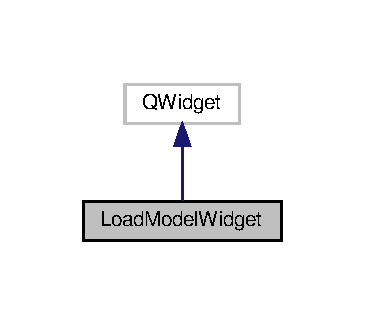
\includegraphics[width=175pt]{classLoadModelWidget__inherit__graph}
\end{center}
\end{figure}


Collaboration diagram for Load\+Model\+Widget\+:\nopagebreak
\begin{figure}[H]
\begin{center}
\leavevmode
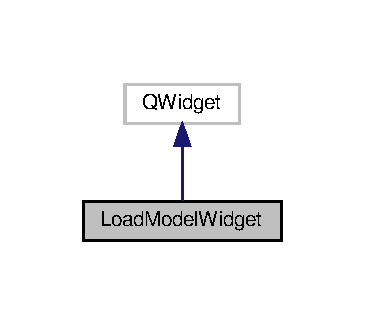
\includegraphics[width=175pt]{classLoadModelWidget__coll__graph}
\end{center}
\end{figure}
\subsection*{Signals}
\begin{DoxyCompactItemize}
\item 
\mbox{\Hypertarget{classLoadModelWidget_a1f2f14a6cfa96c2d4f3524d8ce7c49d7}\label{classLoadModelWidget_a1f2f14a6cfa96c2d4f3524d8ce7c49d7}} 
void \hyperlink{classLoadModelWidget_a1f2f14a6cfa96c2d4f3524d8ce7c49d7}{Load\+Data} (std\+::string const \&file\+\_\+path)
\begin{DoxyCompactList}\small\item\em A signal that is emitted when the load button is clicked. \end{DoxyCompactList}\end{DoxyCompactItemize}
\subsection*{Public Member Functions}
\begin{DoxyCompactItemize}
\item 
\mbox{\Hypertarget{classLoadModelWidget_a1d65aba05b2bcc5f9940cb1fede85b1a}\label{classLoadModelWidget_a1d65aba05b2bcc5f9940cb1fede85b1a}} 
\hyperlink{classLoadModelWidget_a1d65aba05b2bcc5f9940cb1fede85b1a}{Load\+Model\+Widget} ()
\begin{DoxyCompactList}\small\item\em Creates the widget with no file selected. \end{DoxyCompactList}\end{DoxyCompactItemize}


\subsection{Detailed Description}
A widget to select a file from which to load a model. 

Definition at line 11 of file load\+\_\+model\+\_\+widget.\+h.



The documentation for this class was generated from the following files\+:\begin{DoxyCompactItemize}
\item 
G\+U\+I/\+Main\+Window/load\+\_\+model\+\_\+widget.\+h\item 
G\+U\+I/\+Main\+Window/load\+\_\+model\+\_\+widget.\+cpp\end{DoxyCompactItemize}

\hypertarget{classMainWindow}{}\section{Main\+Window Class Reference}
\label{classMainWindow}\index{Main\+Window@{Main\+Window}}


Inheritance diagram for Main\+Window\+:
\nopagebreak
\begin{figure}[H]
\begin{center}
\leavevmode
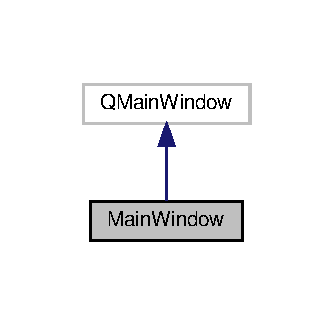
\includegraphics[width=160pt]{classMainWindow__inherit__graph}
\end{center}
\end{figure}


Collaboration diagram for Main\+Window\+:
\nopagebreak
\begin{figure}[H]
\begin{center}
\leavevmode
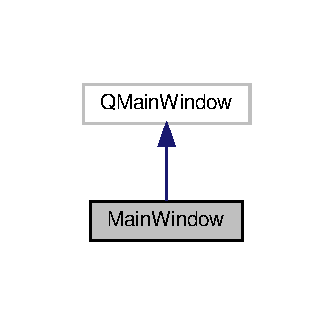
\includegraphics[width=160pt]{classMainWindow__coll__graph}
\end{center}
\end{figure}


The documentation for this class was generated from the following files\+:\begin{DoxyCompactItemize}
\item 
G\+U\+I/main\+\_\+window.\+h\item 
G\+U\+I/main\+\_\+window.\+cpp\end{DoxyCompactItemize}

\hypertarget{classMatrix}{}\section{Matrix Class Reference}
\label{classMatrix}\index{Matrix@{Matrix}}


Represents a matrix with real numbers.  




{\ttfamily \#include $<$matrix.\+h$>$}

\subsection*{Public Member Functions}
\begin{DoxyCompactItemize}
\item 
\mbox{\Hypertarget{classMatrix_a12d35ef1824cd847868a8703035b0d5d}\label{classMatrix_a12d35ef1824cd847868a8703035b0d5d}} 
\hyperlink{classMatrix_a12d35ef1824cd847868a8703035b0d5d}{Matrix} ()=default
\begin{DoxyCompactList}\small\item\em Creates an empty matrix. \end{DoxyCompactList}\item 
\hyperlink{classMatrix_ae157f910061b3e1155b17b62583bde57}{Matrix} (int n, int m)
\item 
\mbox{\Hypertarget{classMatrix_a409518fdf191a193bf544e0148fdc9cc}\label{classMatrix_a409518fdf191a193bf544e0148fdc9cc}} 
int \hyperlink{classMatrix_a409518fdf191a193bf544e0148fdc9cc}{Rows} () const
\begin{DoxyCompactList}\small\item\em Returns the number of rows of the matrix. \end{DoxyCompactList}\item 
\mbox{\Hypertarget{classMatrix_a742ff4cea157cd4d7a1943ddbc702028}\label{classMatrix_a742ff4cea157cd4d7a1943ddbc702028}} 
int \hyperlink{classMatrix_a742ff4cea157cd4d7a1943ddbc702028}{Columns} () const
\begin{DoxyCompactList}\small\item\em Returns the number of columns of the matrix. \end{DoxyCompactList}\item 
\hyperlink{classMatrix}{Matrix} \hyperlink{classMatrix_a2c888c6a7fe7a4ea3b603d17fe3f77e0}{operator+} (\hyperlink{classMatrix}{Matrix} const \&other) const
\item 
\hyperlink{classMatrix}{Matrix} \& \hyperlink{classMatrix_a5f5d62f853a2ed97f2ba437036b1724d}{operator+=} (\hyperlink{classMatrix}{Matrix} const \&other)
\item 
\hyperlink{classMatrix}{Matrix} \hyperlink{classMatrix_a5f7129af600c22b69abdcb2c3b204e5a}{operator-\/} (\hyperlink{classMatrix}{Matrix} const \&other) const
\item 
\hyperlink{classMatrix}{Matrix} \& \hyperlink{classMatrix_a5871f028dc8b3ae8043a942b5840cdec}{operator-\/=} (\hyperlink{classMatrix}{Matrix} const \&other)
\item 
\hyperlink{classMatrix}{Matrix} \hyperlink{classMatrix_a087f5fbe295229d2790871bb14b6a2a5}{operator$\ast$} (\hyperlink{classMatrix}{Matrix} const \&other) const
\item 
\hyperlink{classMatrix}{Matrix} \& \hyperlink{classMatrix_a8d3c514ae15700397053fd3402552b1c}{operator$\ast$=} (\hyperlink{classMatrix}{Matrix} const \&other)
\item 
\hyperlink{classMatrix}{Matrix} \hyperlink{classMatrix_afdd6cdea30961d5ce34be67332c1d0dd}{operator$\ast$} (double other) const
\item 
\hyperlink{classMatrix}{Matrix} \& \hyperlink{classMatrix_ad2fd5772e288eb07a404907e6e1a1dd6}{operator$\ast$=} (double other)
\item 
\hyperlink{classMatrix}{Matrix} \hyperlink{classMatrix_aef843067e6c43218c7c909b6367706c2}{operator\%} (\hyperlink{classMatrix}{Matrix} const \&other) const
\item 
\hyperlink{classMatrix}{Matrix} \& \hyperlink{classMatrix_ac391b0910e9f0fc0a6e23c9346cee2ad}{operator\%=} (\hyperlink{classMatrix}{Matrix} const \&other)
\item 
\mbox{\Hypertarget{classMatrix_ad0c96cdea0d2ae3403653ca90aa70796}\label{classMatrix_ad0c96cdea0d2ae3403653ca90aa70796}} 
\hyperlink{classMatrix}{Matrix} \hyperlink{classMatrix_ad0c96cdea0d2ae3403653ca90aa70796}{Transpose} () const
\begin{DoxyCompactList}\small\item\em Returns the transposed matrix. \end{DoxyCompactList}\item 
\mbox{\Hypertarget{classMatrix_ad5f101877c4a10988bf7f128a9c248d8}\label{classMatrix_ad5f101877c4a10988bf7f128a9c248d8}} 
\hyperlink{classMatrix}{Matrix} \hyperlink{classMatrix_ad5f101877c4a10988bf7f128a9c248d8}{Inverse} () const
\begin{DoxyCompactList}\small\item\em Returns the inverse matrix. \end{DoxyCompactList}\item 
std\+::vector$<$ double $>$ \& \hyperlink{classMatrix_a25cb20c90560327240a07d81ed11c746}{operator\mbox{[}$\,$\mbox{]}} (int row)
\item 
std\+::vector$<$ double $>$ const  \& \hyperlink{classMatrix_a120efaa8b3a945230e8a601927cb0e47}{operator\mbox{[}$\,$\mbox{]}} (int row) const
\end{DoxyCompactItemize}


\subsection{Detailed Description}
Represents a matrix with real numbers. 

\subsection{Constructor \& Destructor Documentation}
\mbox{\Hypertarget{classMatrix_ae157f910061b3e1155b17b62583bde57}\label{classMatrix_ae157f910061b3e1155b17b62583bde57}} 
\index{Matrix@{Matrix}!Matrix@{Matrix}}
\index{Matrix@{Matrix}!Matrix@{Matrix}}
\subsubsection{\texorpdfstring{Matrix()}{Matrix()}}
{\footnotesize\ttfamily Matrix\+::\+Matrix (\begin{DoxyParamCaption}\item[{int}]{n,  }\item[{int}]{m }\end{DoxyParamCaption})}

Creates a matrix of {\ttfamily n} rows and {\ttfamily m} columns.


\begin{DoxyParams}{Parameters}
{\em n} & The number of rows. \\
\hline
{\em m} & The number of columns. \\
\hline
\end{DoxyParams}


\subsection{Member Function Documentation}
\mbox{\Hypertarget{classMatrix_aef843067e6c43218c7c909b6367706c2}\label{classMatrix_aef843067e6c43218c7c909b6367706c2}} 
\index{Matrix@{Matrix}!operator\%@{operator\%}}
\index{operator\%@{operator\%}!Matrix@{Matrix}}
\subsubsection{\texorpdfstring{operator\%()}{operator\%()}}
{\footnotesize\ttfamily \hyperlink{classMatrix}{Matrix} Matrix\+::operator\% (\begin{DoxyParamCaption}\item[{\hyperlink{classMatrix}{Matrix} const \&}]{other }\end{DoxyParamCaption}) const}

Applies the Hadamard product to the object and the matrix {\ttfamily other} and returns the resulting matrix. The object is left unchanges.


\begin{DoxyParams}{Parameters}
{\em other} & The matrix to be multiplied to the object. \\
\hline
\end{DoxyParams}
\mbox{\Hypertarget{classMatrix_ac391b0910e9f0fc0a6e23c9346cee2ad}\label{classMatrix_ac391b0910e9f0fc0a6e23c9346cee2ad}} 
\index{Matrix@{Matrix}!operator\%=@{operator\%=}}
\index{operator\%=@{operator\%=}!Matrix@{Matrix}}
\subsubsection{\texorpdfstring{operator\%=()}{operator\%=()}}
{\footnotesize\ttfamily \hyperlink{classMatrix}{Matrix} \& Matrix\+::operator\%= (\begin{DoxyParamCaption}\item[{\hyperlink{classMatrix}{Matrix} const \&}]{other }\end{DoxyParamCaption})}

Applies the Hadamard product to the object and the matrix {\ttfamily other} and overwrites the current value of the object.


\begin{DoxyParams}{Parameters}
{\em other} & The matrix to be multiplied to the object. \\
\hline
\end{DoxyParams}
\mbox{\Hypertarget{classMatrix_a087f5fbe295229d2790871bb14b6a2a5}\label{classMatrix_a087f5fbe295229d2790871bb14b6a2a5}} 
\index{Matrix@{Matrix}!operator$\ast$@{operator$\ast$}}
\index{operator$\ast$@{operator$\ast$}!Matrix@{Matrix}}
\subsubsection{\texorpdfstring{operator$\ast$()}{operator*()}\hspace{0.1cm}{\footnotesize\ttfamily [1/2]}}
{\footnotesize\ttfamily \hyperlink{classMatrix}{Matrix} Matrix\+::operator$\ast$ (\begin{DoxyParamCaption}\item[{\hyperlink{classMatrix}{Matrix} const \&}]{other }\end{DoxyParamCaption}) const}

Multiplies the matrix {\ttfamily other} to this object and returns the resulting matrix. The object is left unchanged.


\begin{DoxyParams}{Parameters}
{\em other} & The matrix to be multiplied to the object. \\
\hline
\end{DoxyParams}
\mbox{\Hypertarget{classMatrix_afdd6cdea30961d5ce34be67332c1d0dd}\label{classMatrix_afdd6cdea30961d5ce34be67332c1d0dd}} 
\index{Matrix@{Matrix}!operator$\ast$@{operator$\ast$}}
\index{operator$\ast$@{operator$\ast$}!Matrix@{Matrix}}
\subsubsection{\texorpdfstring{operator$\ast$()}{operator*()}\hspace{0.1cm}{\footnotesize\ttfamily [2/2]}}
{\footnotesize\ttfamily \hyperlink{classMatrix}{Matrix} Matrix\+::operator$\ast$ (\begin{DoxyParamCaption}\item[{double}]{other }\end{DoxyParamCaption}) const}

Multiplies the real number {\ttfamily other} to this object and returns the resulting matrix. The object is left unchanged.


\begin{DoxyParams}{Parameters}
{\em other} & The real number to be multiplied to the object. \\
\hline
\end{DoxyParams}
\mbox{\Hypertarget{classMatrix_a8d3c514ae15700397053fd3402552b1c}\label{classMatrix_a8d3c514ae15700397053fd3402552b1c}} 
\index{Matrix@{Matrix}!operator$\ast$=@{operator$\ast$=}}
\index{operator$\ast$=@{operator$\ast$=}!Matrix@{Matrix}}
\subsubsection{\texorpdfstring{operator$\ast$=()}{operator*=()}\hspace{0.1cm}{\footnotesize\ttfamily [1/2]}}
{\footnotesize\ttfamily \hyperlink{classMatrix}{Matrix} \& Matrix\+::operator$\ast$= (\begin{DoxyParamCaption}\item[{\hyperlink{classMatrix}{Matrix} const \&}]{other }\end{DoxyParamCaption})}

Multiplies the matrix {\ttfamily other} into this object.


\begin{DoxyParams}{Parameters}
{\em other} & The matrix to be multiplied to the object. \\
\hline
\end{DoxyParams}
\mbox{\Hypertarget{classMatrix_ad2fd5772e288eb07a404907e6e1a1dd6}\label{classMatrix_ad2fd5772e288eb07a404907e6e1a1dd6}} 
\index{Matrix@{Matrix}!operator$\ast$=@{operator$\ast$=}}
\index{operator$\ast$=@{operator$\ast$=}!Matrix@{Matrix}}
\subsubsection{\texorpdfstring{operator$\ast$=()}{operator*=()}\hspace{0.1cm}{\footnotesize\ttfamily [2/2]}}
{\footnotesize\ttfamily \hyperlink{classMatrix}{Matrix} \& Matrix\+::operator$\ast$= (\begin{DoxyParamCaption}\item[{double}]{other }\end{DoxyParamCaption})}

Multiplies the real number {\ttfamily other} into this object.


\begin{DoxyParams}{Parameters}
{\em other} & The real number to be multiplied to the object. \\
\hline
\end{DoxyParams}
\mbox{\Hypertarget{classMatrix_a2c888c6a7fe7a4ea3b603d17fe3f77e0}\label{classMatrix_a2c888c6a7fe7a4ea3b603d17fe3f77e0}} 
\index{Matrix@{Matrix}!operator+@{operator+}}
\index{operator+@{operator+}!Matrix@{Matrix}}
\subsubsection{\texorpdfstring{operator+()}{operator+()}}
{\footnotesize\ttfamily \hyperlink{classMatrix}{Matrix} Matrix\+::operator+ (\begin{DoxyParamCaption}\item[{\hyperlink{classMatrix}{Matrix} const \&}]{other }\end{DoxyParamCaption}) const}

Adds the matrix {\ttfamily other} to this object and returns the resulting matrix. The object is left unchanged.


\begin{DoxyParams}{Parameters}
{\em other} & The matrix to be added to the object. \\
\hline
\end{DoxyParams}
\mbox{\Hypertarget{classMatrix_a5f5d62f853a2ed97f2ba437036b1724d}\label{classMatrix_a5f5d62f853a2ed97f2ba437036b1724d}} 
\index{Matrix@{Matrix}!operator+=@{operator+=}}
\index{operator+=@{operator+=}!Matrix@{Matrix}}
\subsubsection{\texorpdfstring{operator+=()}{operator+=()}}
{\footnotesize\ttfamily \hyperlink{classMatrix}{Matrix} \& Matrix\+::operator+= (\begin{DoxyParamCaption}\item[{\hyperlink{classMatrix}{Matrix} const \&}]{other }\end{DoxyParamCaption})}

Adds the matrix {\ttfamily other} into this object.


\begin{DoxyParams}{Parameters}
{\em other} & The matrix to be added to the object. \\
\hline
\end{DoxyParams}
\mbox{\Hypertarget{classMatrix_a5f7129af600c22b69abdcb2c3b204e5a}\label{classMatrix_a5f7129af600c22b69abdcb2c3b204e5a}} 
\index{Matrix@{Matrix}!operator-\/@{operator-\/}}
\index{operator-\/@{operator-\/}!Matrix@{Matrix}}
\subsubsection{\texorpdfstring{operator-\/()}{operator-()}}
{\footnotesize\ttfamily \hyperlink{classMatrix}{Matrix} Matrix\+::operator-\/ (\begin{DoxyParamCaption}\item[{\hyperlink{classMatrix}{Matrix} const \&}]{other }\end{DoxyParamCaption}) const}

Subtracts the matrix {\ttfamily other} to this object and returns the resulting matrix. The object is left unchanged.


\begin{DoxyParams}{Parameters}
{\em other} & The matrix to be subtracted to the object. \\
\hline
\end{DoxyParams}
\mbox{\Hypertarget{classMatrix_a5871f028dc8b3ae8043a942b5840cdec}\label{classMatrix_a5871f028dc8b3ae8043a942b5840cdec}} 
\index{Matrix@{Matrix}!operator-\/=@{operator-\/=}}
\index{operator-\/=@{operator-\/=}!Matrix@{Matrix}}
\subsubsection{\texorpdfstring{operator-\/=()}{operator-=()}}
{\footnotesize\ttfamily \hyperlink{classMatrix}{Matrix} \& Matrix\+::operator-\/= (\begin{DoxyParamCaption}\item[{\hyperlink{classMatrix}{Matrix} const \&}]{other }\end{DoxyParamCaption})}

Subtracts the matrix {\ttfamily other} into this object.


\begin{DoxyParams}{Parameters}
{\em other} & The matrix to be subtracted to the object. \\
\hline
\end{DoxyParams}
\mbox{\Hypertarget{classMatrix_a25cb20c90560327240a07d81ed11c746}\label{classMatrix_a25cb20c90560327240a07d81ed11c746}} 
\index{Matrix@{Matrix}!operator\mbox{[}\mbox{]}@{operator[]}}
\index{operator\mbox{[}\mbox{]}@{operator[]}!Matrix@{Matrix}}
\subsubsection{\texorpdfstring{operator[]()}{operator[]()}\hspace{0.1cm}{\footnotesize\ttfamily [1/2]}}
{\footnotesize\ttfamily std\+::vector$<$double$>$\& Matrix\+::operator\mbox{[}$\,$\mbox{]} (\begin{DoxyParamCaption}\item[{int}]{row }\end{DoxyParamCaption})\hspace{0.3cm}{\ttfamily [inline]}}

Returns the row of numbers indicated by {\ttfamily row}.


\begin{DoxyParams}{Parameters}
{\em row} & The index of the row. \\
\hline
\end{DoxyParams}
\mbox{\Hypertarget{classMatrix_a120efaa8b3a945230e8a601927cb0e47}\label{classMatrix_a120efaa8b3a945230e8a601927cb0e47}} 
\index{Matrix@{Matrix}!operator\mbox{[}\mbox{]}@{operator[]}}
\index{operator\mbox{[}\mbox{]}@{operator[]}!Matrix@{Matrix}}
\subsubsection{\texorpdfstring{operator[]()}{operator[]()}\hspace{0.1cm}{\footnotesize\ttfamily [2/2]}}
{\footnotesize\ttfamily std\+::vector$<$double$>$ const\& Matrix\+::operator\mbox{[}$\,$\mbox{]} (\begin{DoxyParamCaption}\item[{int}]{row }\end{DoxyParamCaption}) const\hspace{0.3cm}{\ttfamily [inline]}}

Returns the row of numbers indicated by {\ttfamily row}.


\begin{DoxyParams}{Parameters}
{\em row} & The index of the row. \\
\hline
\end{DoxyParams}


The documentation for this class was generated from the following files\+:\begin{DoxyCompactItemize}
\item 
Utils/matrix.\+h\item 
Utils/matrix.\+cpp\end{DoxyCompactItemize}

\hypertarget{classMergeDialog}{}\section{Merge\+Dialog Class Reference}
\label{classMergeDialog}\index{Merge\+Dialog@{Merge\+Dialog}}


Inheritance diagram for Merge\+Dialog\+:
\nopagebreak
\begin{figure}[H]
\begin{center}
\leavevmode
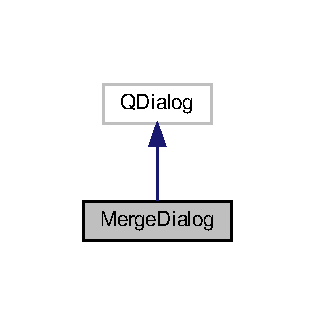
\includegraphics[width=151pt]{classMergeDialog__inherit__graph}
\end{center}
\end{figure}


Collaboration diagram for Merge\+Dialog\+:
\nopagebreak
\begin{figure}[H]
\begin{center}
\leavevmode
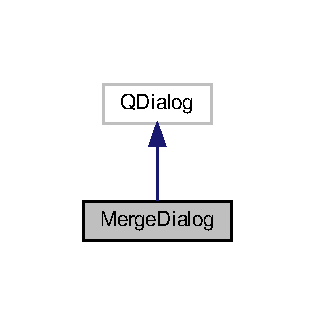
\includegraphics[width=151pt]{classMergeDialog__coll__graph}
\end{center}
\end{figure}
\subsection*{Public Member Functions}
\begin{DoxyCompactItemize}
\item 
\mbox{\Hypertarget{classMergeDialog_ae95937aa77ed7551b9b7cc7b9a148180}\label{classMergeDialog_ae95937aa77ed7551b9b7cc7b9a148180}} 
{\bfseries Merge\+Dialog} (Q\+Widget $\ast$parent, \hyperlink{classModelInterface}{Model\+Interface} const \&model)
\end{DoxyCompactItemize}


\subsection{Detailed Description}


Definition at line 8 of file merge\+\_\+dialog.\+h.



The documentation for this class was generated from the following files\+:\begin{DoxyCompactItemize}
\item 
G\+U\+I/\+Model\+Window/\+Merge\+Dialog/merge\+\_\+dialog.\+h\item 
G\+U\+I/\+Model\+Window/\+Merge\+Dialog/merge\+\_\+dialog.\+cpp\end{DoxyCompactItemize}

\hypertarget{classMergeWidget}{}\section{Merge\+Widget Class Reference}
\label{classMergeWidget}\index{Merge\+Widget@{Merge\+Widget}}


Inheritance diagram for Merge\+Widget\+:
\nopagebreak
\begin{figure}[H]
\begin{center}
\leavevmode
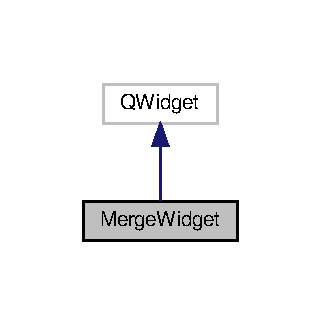
\includegraphics[width=154pt]{classMergeWidget__inherit__graph}
\end{center}
\end{figure}


Collaboration diagram for Merge\+Widget\+:
\nopagebreak
\begin{figure}[H]
\begin{center}
\leavevmode
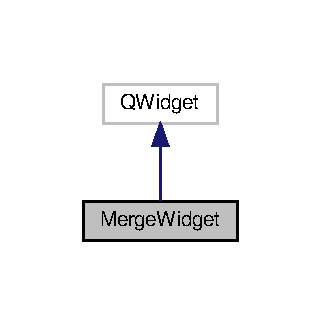
\includegraphics[width=154pt]{classMergeWidget__coll__graph}
\end{center}
\end{figure}
\subsection*{Public Member Functions}
\begin{DoxyCompactItemize}
\item 
\mbox{\Hypertarget{classMergeWidget_a4974b0fd859f7e6b91a5839d8245901b}\label{classMergeWidget_a4974b0fd859f7e6b91a5839d8245901b}} 
{\bfseries Merge\+Widget} (Q\+Widget $\ast$parent, \hyperlink{classModelInterface}{Model\+Interface} const \&model)
\end{DoxyCompactItemize}


\subsection{Detailed Description}


Definition at line 9 of file merge\+\_\+widget.\+h.



The documentation for this class was generated from the following files\+:\begin{DoxyCompactItemize}
\item 
G\+U\+I/\+Model\+Window/\+Merge\+Dialog/merge\+\_\+widget.\+h\item 
G\+U\+I/\+Model\+Window/\+Merge\+Dialog/merge\+\_\+widget.\+cpp\end{DoxyCompactItemize}

\hypertarget{classModelFactory}{}\section{Model\+Factory Class Reference}
\label{classModelFactory}\index{Model\+Factory@{Model\+Factory}}
\subsection*{Static Public Member Functions}
\begin{DoxyCompactItemize}
\item 
\mbox{\Hypertarget{classModelFactory_aedb972860999dae2693b1f6a1c8fe920}\label{classModelFactory_aedb972860999dae2693b1f6a1c8fe920}} 
static std\+::unique\+\_\+ptr$<$ \hyperlink{classModelInterface}{Model\+Interface} $>$ {\bfseries Create\+Model} (std\+::string const \&file\+\_\+name, Model\+Type model\+\_\+type)
\end{DoxyCompactItemize}


\subsection{Detailed Description}


Definition at line 7 of file model\+\_\+factory.\+h.



The documentation for this class was generated from the following file\+:\begin{DoxyCompactItemize}
\item 
Models/model\+\_\+factory.\+h\end{DoxyCompactItemize}

\hypertarget{classModelInterface}{}\section{Model\+Interface Class Reference}
\label{classModelInterface}\index{Model\+Interface@{Model\+Interface}}


An interface for any model.  




{\ttfamily \#include $<$model\+\_\+interface.\+h$>$}



Inheritance diagram for Model\+Interface\+:
\nopagebreak
\begin{figure}[H]
\begin{center}
\leavevmode
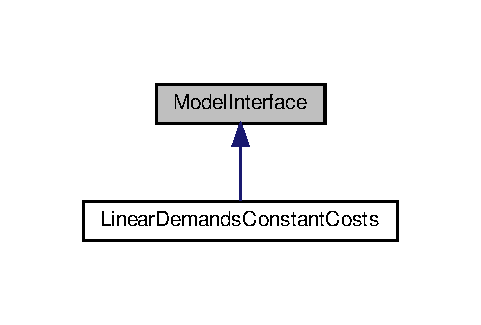
\includegraphics[width=231pt]{classModelInterface__inherit__graph}
\end{center}
\end{figure}
\subsection*{Public Member Functions}
\begin{DoxyCompactItemize}
\item 
\mbox{\Hypertarget{classModelInterface_ad2d37b05bed8ef0663a4e75221c31e7d}\label{classModelInterface_ad2d37b05bed8ef0663a4e75221c31e7d}} 
virtual std\+::string \hyperlink{classModelInterface_ad2d37b05bed8ef0663a4e75221c31e7d}{Get\+Name} () const =0
\begin{DoxyCompactList}\small\item\em Returns the name of the model. \end{DoxyCompactList}\item 
\mbox{\Hypertarget{classModelInterface_abb173c60dc16ba8b0e087f8edbbeb5b9}\label{classModelInterface_abb173c60dc16ba8b0e087f8edbbeb5b9}} 
virtual int \hyperlink{classModelInterface_abb173c60dc16ba8b0e087f8edbbeb5b9}{Get\+Number\+Of\+Products} () const =0
\begin{DoxyCompactList}\small\item\em Returns the number of products. \end{DoxyCompactList}\item 
\mbox{\Hypertarget{classModelInterface_adc2c55b551054c0a98869bc0497919a8}\label{classModelInterface_adc2c55b551054c0a98869bc0497919a8}} 
virtual \hyperlink{classColumnVector}{Column\+Vector} \hyperlink{classModelInterface_adc2c55b551054c0a98869bc0497919a8}{Compute\+Prices} () const =0
\begin{DoxyCompactList}\small\item\em Computes the equilibrium prices of the model. \end{DoxyCompactList}\item 
virtual \hyperlink{classColumnVector}{Column\+Vector} \hyperlink{classModelInterface_af9a936f6f0d1b1f0f2c5bf35785e7db4}{Compute\+Quantities} (\hyperlink{classColumnVector}{Column\+Vector} const \&prices) const =0
\item 
virtual \hyperlink{classColumnVector}{Column\+Vector} \hyperlink{classModelInterface_ac0a7cc3db9fc177dc75f16abf00275a7}{Compute\+Costs} (\hyperlink{classColumnVector}{Column\+Vector} const \&quantities) const =0
\item 
virtual \hyperlink{classColumnVector}{Column\+Vector} \hyperlink{classModelInterface_a311a000060cece8fc1058cd27bf07864}{Compute\+Profits} (\hyperlink{classColumnVector}{Column\+Vector} const \&prices) const =0
\item 
virtual \hyperlink{classColumnVector}{Column\+Vector} \hyperlink{classModelInterface_a094ebb85618fb13bf38f6faff1f5dd7b}{Compute\+Consumer\+Welfare} (\hyperlink{classColumnVector}{Column\+Vector} const \&prices) const =0
\item 
virtual void \hyperlink{classModelInterface_a9aa52643da1fe9e74750e31a6c6ec469}{Merge} (int i, int j)=0
\item 
virtual void \hyperlink{classModelInterface_ab5709db8ecb96fd9efd02f4777d5502a}{Save\+To\+File} (std\+::string const \&file\+\_\+path) const =0
\item 
virtual void \hyperlink{classModelInterface_a7f408fdb15c10ce8cabf6b942bbc9c38}{Load\+From\+File} (std\+::string const \&file\+\_\+path)=0
\end{DoxyCompactItemize}


\subsection{Detailed Description}
An interface for any model. 

\subsection{Member Function Documentation}
\mbox{\Hypertarget{classModelInterface_a094ebb85618fb13bf38f6faff1f5dd7b}\label{classModelInterface_a094ebb85618fb13bf38f6faff1f5dd7b}} 
\index{Model\+Interface@{Model\+Interface}!Compute\+Consumer\+Welfare@{Compute\+Consumer\+Welfare}}
\index{Compute\+Consumer\+Welfare@{Compute\+Consumer\+Welfare}!Model\+Interface@{Model\+Interface}}
\subsubsection{\texorpdfstring{Compute\+Consumer\+Welfare()}{ComputeConsumerWelfare()}}
{\footnotesize\ttfamily virtual \hyperlink{classColumnVector}{Column\+Vector} Model\+Interface\+::\+Compute\+Consumer\+Welfare (\begin{DoxyParamCaption}\item[{\hyperlink{classColumnVector}{Column\+Vector} const \&}]{prices }\end{DoxyParamCaption}) const\hspace{0.3cm}{\ttfamily [pure virtual]}}

Computes the consumer welfare of the model in equilibrium.


\begin{DoxyParams}{Parameters}
{\em prices} & The equilibrium prices. \\
\hline
\end{DoxyParams}


Implemented in \hyperlink{classLinearDemandsConstantCosts_a9d3fa6a3b151c2f1703f23bbee6954cb}{Linear\+Demands\+Constant\+Costs}.

\mbox{\Hypertarget{classModelInterface_ac0a7cc3db9fc177dc75f16abf00275a7}\label{classModelInterface_ac0a7cc3db9fc177dc75f16abf00275a7}} 
\index{Model\+Interface@{Model\+Interface}!Compute\+Costs@{Compute\+Costs}}
\index{Compute\+Costs@{Compute\+Costs}!Model\+Interface@{Model\+Interface}}
\subsubsection{\texorpdfstring{Compute\+Costs()}{ComputeCosts()}}
{\footnotesize\ttfamily virtual \hyperlink{classColumnVector}{Column\+Vector} Model\+Interface\+::\+Compute\+Costs (\begin{DoxyParamCaption}\item[{\hyperlink{classColumnVector}{Column\+Vector} const \&}]{quantities }\end{DoxyParamCaption}) const\hspace{0.3cm}{\ttfamily [pure virtual]}}

Computes the costs of the model in equilibrium.


\begin{DoxyParams}{Parameters}
{\em quantities} & The equilibrium quantities. \\
\hline
\end{DoxyParams}


Implemented in \hyperlink{classLinearDemandsConstantCosts_a55e0f15cfc00d8c21fbfd95843c06c44}{Linear\+Demands\+Constant\+Costs}.

\mbox{\Hypertarget{classModelInterface_a311a000060cece8fc1058cd27bf07864}\label{classModelInterface_a311a000060cece8fc1058cd27bf07864}} 
\index{Model\+Interface@{Model\+Interface}!Compute\+Profits@{Compute\+Profits}}
\index{Compute\+Profits@{Compute\+Profits}!Model\+Interface@{Model\+Interface}}
\subsubsection{\texorpdfstring{Compute\+Profits()}{ComputeProfits()}}
{\footnotesize\ttfamily virtual \hyperlink{classColumnVector}{Column\+Vector} Model\+Interface\+::\+Compute\+Profits (\begin{DoxyParamCaption}\item[{\hyperlink{classColumnVector}{Column\+Vector} const \&}]{prices }\end{DoxyParamCaption}) const\hspace{0.3cm}{\ttfamily [pure virtual]}}

Computes the profits of the model in equilibrium.


\begin{DoxyParams}{Parameters}
{\em prices} & The equilibrium prices. \\
\hline
\end{DoxyParams}


Implemented in \hyperlink{classLinearDemandsConstantCosts_a48b52dab01d2cf45beae51eab615f7ae}{Linear\+Demands\+Constant\+Costs}.

\mbox{\Hypertarget{classModelInterface_af9a936f6f0d1b1f0f2c5bf35785e7db4}\label{classModelInterface_af9a936f6f0d1b1f0f2c5bf35785e7db4}} 
\index{Model\+Interface@{Model\+Interface}!Compute\+Quantities@{Compute\+Quantities}}
\index{Compute\+Quantities@{Compute\+Quantities}!Model\+Interface@{Model\+Interface}}
\subsubsection{\texorpdfstring{Compute\+Quantities()}{ComputeQuantities()}}
{\footnotesize\ttfamily virtual \hyperlink{classColumnVector}{Column\+Vector} Model\+Interface\+::\+Compute\+Quantities (\begin{DoxyParamCaption}\item[{\hyperlink{classColumnVector}{Column\+Vector} const \&}]{prices }\end{DoxyParamCaption}) const\hspace{0.3cm}{\ttfamily [pure virtual]}}

Computes the equilibrium quantities of the model.


\begin{DoxyParams}{Parameters}
{\em prices} & The equilibrium prices. \\
\hline
\end{DoxyParams}


Implemented in \hyperlink{classLinearDemandsConstantCosts_a310864e458935098502561540a71a88c}{Linear\+Demands\+Constant\+Costs}.

\mbox{\Hypertarget{classModelInterface_a7f408fdb15c10ce8cabf6b942bbc9c38}\label{classModelInterface_a7f408fdb15c10ce8cabf6b942bbc9c38}} 
\index{Model\+Interface@{Model\+Interface}!Load\+From\+File@{Load\+From\+File}}
\index{Load\+From\+File@{Load\+From\+File}!Model\+Interface@{Model\+Interface}}
\subsubsection{\texorpdfstring{Load\+From\+File()}{LoadFromFile()}}
{\footnotesize\ttfamily virtual void Model\+Interface\+::\+Load\+From\+File (\begin{DoxyParamCaption}\item[{std\+::string const \&}]{file\+\_\+path }\end{DoxyParamCaption})\hspace{0.3cm}{\ttfamily [pure virtual]}}

Loads the model values from the given file path.


\begin{DoxyParams}{Parameters}
{\em file\+\_\+path} & The path of the file from where the model has to read its values. \\
\hline
\end{DoxyParams}


Implemented in \hyperlink{classLinearDemandsConstantCosts_a075add461e368629b9dfd8f72033e2ad}{Linear\+Demands\+Constant\+Costs}.

\mbox{\Hypertarget{classModelInterface_a9aa52643da1fe9e74750e31a6c6ec469}\label{classModelInterface_a9aa52643da1fe9e74750e31a6c6ec469}} 
\index{Model\+Interface@{Model\+Interface}!Merge@{Merge}}
\index{Merge@{Merge}!Model\+Interface@{Model\+Interface}}
\subsubsection{\texorpdfstring{Merge()}{Merge()}}
{\footnotesize\ttfamily virtual void Model\+Interface\+::\+Merge (\begin{DoxyParamCaption}\item[{int}]{i,  }\item[{int}]{j }\end{DoxyParamCaption})\hspace{0.3cm}{\ttfamily [pure virtual]}}

Merges two different firms.


\begin{DoxyParams}{Parameters}
{\em i} & The index of the first firm to merge. \\
\hline
{\em j} & The index of the second firm to merge. \\
\hline
\end{DoxyParams}


Implemented in \hyperlink{classLinearDemandsConstantCosts_a0ee422d927b5a85f9aba8782b02f537b}{Linear\+Demands\+Constant\+Costs}.

\mbox{\Hypertarget{classModelInterface_ab5709db8ecb96fd9efd02f4777d5502a}\label{classModelInterface_ab5709db8ecb96fd9efd02f4777d5502a}} 
\index{Model\+Interface@{Model\+Interface}!Save\+To\+File@{Save\+To\+File}}
\index{Save\+To\+File@{Save\+To\+File}!Model\+Interface@{Model\+Interface}}
\subsubsection{\texorpdfstring{Save\+To\+File()}{SaveToFile()}}
{\footnotesize\ttfamily virtual void Model\+Interface\+::\+Save\+To\+File (\begin{DoxyParamCaption}\item[{std\+::string const \&}]{file\+\_\+path }\end{DoxyParamCaption}) const\hspace{0.3cm}{\ttfamily [pure virtual]}}

Saves the current model values to the given file path.


\begin{DoxyParams}{Parameters}
{\em file\+\_\+path} & The path of the file to where the model will be saved. \\
\hline
\end{DoxyParams}


Implemented in \hyperlink{classLinearDemandsConstantCosts_aef2823751866a4933a8611dd4622d78b}{Linear\+Demands\+Constant\+Costs}.



The documentation for this class was generated from the following file\+:\begin{DoxyCompactItemize}
\item 
Models/model\+\_\+interface.\+h\end{DoxyCompactItemize}

\hypertarget{classModelTableData}{}\section{Model\+Table\+Data Class Reference}
\label{classModelTableData}\index{Model\+Table\+Data@{Model\+Table\+Data}}


Inheritance diagram for Model\+Table\+Data\+:\nopagebreak
\begin{figure}[H]
\begin{center}
\leavevmode
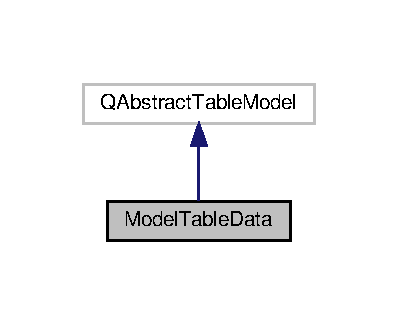
\includegraphics[width=191pt]{classModelTableData__inherit__graph}
\end{center}
\end{figure}


Collaboration diagram for Model\+Table\+Data\+:\nopagebreak
\begin{figure}[H]
\begin{center}
\leavevmode
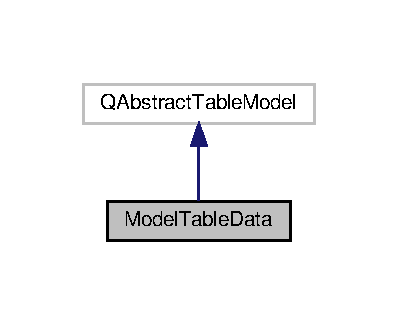
\includegraphics[width=191pt]{classModelTableData__coll__graph}
\end{center}
\end{figure}
\subsection*{Public Member Functions}
\begin{DoxyCompactItemize}
\item 
\mbox{\Hypertarget{classModelTableData_a55b75d87fd591b326fb3deb130f2a981}\label{classModelTableData_a55b75d87fd591b326fb3deb130f2a981}} 
{\bfseries Model\+Table\+Data} (std\+::string const \&file\+\_\+path, Model\+Type model\+\_\+type)
\item 
\mbox{\Hypertarget{classModelTableData_ad74b4571c5eb8bf2f84d16392f0885a8}\label{classModelTableData_ad74b4571c5eb8bf2f84d16392f0885a8}} 
virtual int {\bfseries row\+Count} (Q\+Model\+Index const \&parent) const override final
\item 
\mbox{\Hypertarget{classModelTableData_a269f93a13692b67fe9513433b02ec1ef}\label{classModelTableData_a269f93a13692b67fe9513433b02ec1ef}} 
virtual int {\bfseries column\+Count} (Q\+Model\+Index const \&parent) const override final
\item 
\mbox{\Hypertarget{classModelTableData_a8e9e7be0b67bdefc68b5fe6b05c38acf}\label{classModelTableData_a8e9e7be0b67bdefc68b5fe6b05c38acf}} 
virtual Q\+Variant {\bfseries data} (Q\+Model\+Index const \&index, int role) const override final
\item 
\mbox{\Hypertarget{classModelTableData_a86985a36d748a7cf35302d8a0c63752a}\label{classModelTableData_a86985a36d748a7cf35302d8a0c63752a}} 
virtual Q\+Variant {\bfseries header\+Data} (int section, Qt\+::\+Orientation orientation, int role) const override final
\end{DoxyCompactItemize}


\subsection{Detailed Description}


Definition at line 9 of file model\+\_\+table\+\_\+data.\+h.



The documentation for this class was generated from the following files\+:\begin{DoxyCompactItemize}
\item 
G\+U\+I/\+Model\+Window/model\+\_\+table\+\_\+data.\+h\item 
G\+U\+I/\+Model\+Window/model\+\_\+table\+\_\+data.\+cpp\end{DoxyCompactItemize}

\hypertarget{classModelTableView}{}\section{Model\+Table\+View Class Reference}
\label{classModelTableView}\index{Model\+Table\+View@{Model\+Table\+View}}


Inheritance diagram for Model\+Table\+View\+:\nopagebreak
\begin{figure}[H]
\begin{center}
\leavevmode
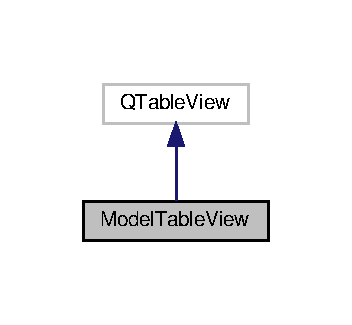
\includegraphics[width=169pt]{classModelTableView__inherit__graph}
\end{center}
\end{figure}


Collaboration diagram for Model\+Table\+View\+:\nopagebreak
\begin{figure}[H]
\begin{center}
\leavevmode
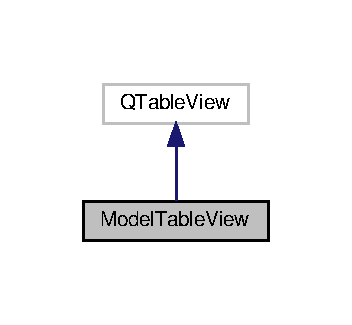
\includegraphics[width=169pt]{classModelTableView__coll__graph}
\end{center}
\end{figure}
\subsection*{Public Member Functions}
\begin{DoxyCompactItemize}
\item 
\mbox{\Hypertarget{classModelTableView_a064d6950aeb8a512fbd0557e3926ecf3}\label{classModelTableView_a064d6950aeb8a512fbd0557e3926ecf3}} 
{\bfseries Model\+Table\+View} (Q\+Widget $\ast$parent, std\+::string const \&file\+\_\+path, Model\+Type model\+\_\+type)
\end{DoxyCompactItemize}
\subsection*{Protected Member Functions}
\begin{DoxyCompactItemize}
\item 
\mbox{\Hypertarget{classModelTableView_a8624c6f242a68c23550dcd5e95277781}\label{classModelTableView_a8624c6f242a68c23550dcd5e95277781}} 
virtual void {\bfseries key\+Press\+Event} (Q\+Key\+Event $\ast$event) override final
\item 
\mbox{\Hypertarget{classModelTableView_a234ac535e1561096114f2c4a05331282}\label{classModelTableView_a234ac535e1561096114f2c4a05331282}} 
virtual Q\+Size {\bfseries size\+Hint} () const override final
\end{DoxyCompactItemize}


\subsection{Detailed Description}


Definition at line 9 of file model\+\_\+table\+\_\+view.\+h.



The documentation for this class was generated from the following files\+:\begin{DoxyCompactItemize}
\item 
G\+U\+I/\+Model\+Window/model\+\_\+table\+\_\+view.\+h\item 
G\+U\+I/\+Model\+Window/model\+\_\+table\+\_\+view.\+cpp\end{DoxyCompactItemize}

\hypertarget{classModelWindow}{}\section{Model\+Window Class Reference}
\label{classModelWindow}\index{Model\+Window@{Model\+Window}}


Inheritance diagram for Model\+Window\+:\nopagebreak
\begin{figure}[H]
\begin{center}
\leavevmode
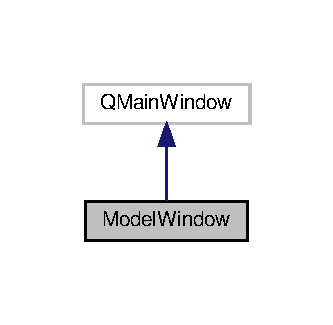
\includegraphics[width=160pt]{classModelWindow__inherit__graph}
\end{center}
\end{figure}


Collaboration diagram for Model\+Window\+:\nopagebreak
\begin{figure}[H]
\begin{center}
\leavevmode
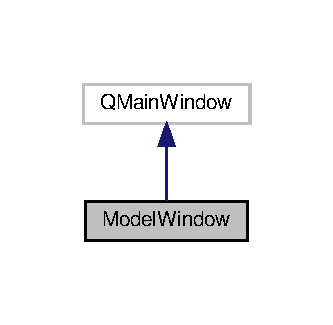
\includegraphics[width=160pt]{classModelWindow__coll__graph}
\end{center}
\end{figure}
\subsection*{Public Member Functions}
\begin{DoxyCompactItemize}
\item 
\mbox{\Hypertarget{classModelWindow_a6035f5f05a539e4bc3593837e60c700f}\label{classModelWindow_a6035f5f05a539e4bc3593837e60c700f}} 
{\bfseries Model\+Window} (Q\+Widget $\ast$parent, std\+::string const \&file\+\_\+path, Model\+Type model\+\_\+type, int model\+\_\+index, std\+::vector$<$ \hyperlink{classModelWindow}{Model\+Window} $\ast$$>$ \&model\+\_\+windows)
\end{DoxyCompactItemize}


\subsection{Detailed Description}


Definition at line 11 of file model\+\_\+window.\+h.



The documentation for this class was generated from the following files\+:\begin{DoxyCompactItemize}
\item 
G\+U\+I/\+Model\+Window/model\+\_\+window.\+h\item 
G\+U\+I/\+Model\+Window/model\+\_\+window.\+cpp\end{DoxyCompactItemize}

\hypertarget{classMultiProductFirmsWidget}{}\section{Multi\+Product\+Firms\+Widget Class Reference}
\label{classMultiProductFirmsWidget}\index{Multi\+Product\+Firms\+Widget@{Multi\+Product\+Firms\+Widget}}


Inheritance diagram for Multi\+Product\+Firms\+Widget\+:
\nopagebreak
\begin{figure}[H]
\begin{center}
\leavevmode
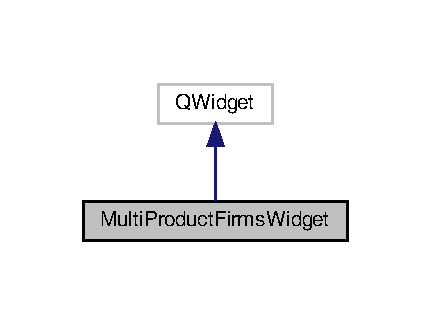
\includegraphics[width=207pt]{classMultiProductFirmsWidget__inherit__graph}
\end{center}
\end{figure}


Collaboration diagram for Multi\+Product\+Firms\+Widget\+:
\nopagebreak
\begin{figure}[H]
\begin{center}
\leavevmode
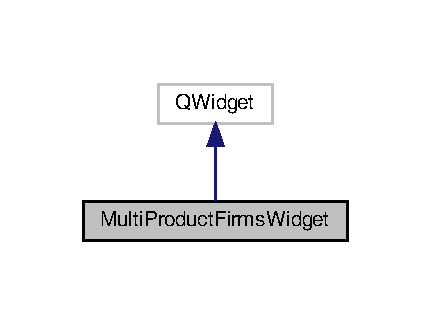
\includegraphics[width=207pt]{classMultiProductFirmsWidget__coll__graph}
\end{center}
\end{figure}
\subsection*{Public Member Functions}
\begin{DoxyCompactItemize}
\item 
\mbox{\Hypertarget{classMultiProductFirmsWidget_a08715f8dd7f9d2bbe0a3686aa41e9462}\label{classMultiProductFirmsWidget_a08715f8dd7f9d2bbe0a3686aa41e9462}} 
{\bfseries Multi\+Product\+Firms\+Widget} (Q\+Widget $\ast$parent)
\end{DoxyCompactItemize}


\subsection{Detailed Description}


Definition at line 9 of file multi\+\_\+product\+\_\+firms\+\_\+widget.\+h.



The documentation for this class was generated from the following files\+:\begin{DoxyCompactItemize}
\item 
G\+U\+I/\+Model\+Window/\+Merge\+Dialog/\+Helpers/multi\+\_\+product\+\_\+firms\+\_\+widget.\+h\item 
G\+U\+I/\+Model\+Window/\+Merge\+Dialog/\+Helpers/multi\+\_\+product\+\_\+firms\+\_\+widget.\+cpp\end{DoxyCompactItemize}

\hypertarget{classRowVector}{}\section{Row\+Vector Class Reference}
\label{classRowVector}\index{Row\+Vector@{Row\+Vector}}
\subsection*{Public Member Functions}
\begin{DoxyCompactItemize}
\item 
\mbox{\Hypertarget{classRowVector_a5996e3aced7d8763c45878e92d1f349f}\label{classRowVector_a5996e3aced7d8763c45878e92d1f349f}} 
{\bfseries Row\+Vector} (int n)
\item 
\mbox{\Hypertarget{classRowVector_a908702c4391bbc161aa6772f0d54c8ee}\label{classRowVector_a908702c4391bbc161aa6772f0d54c8ee}} 
int {\bfseries Size} () const
\item 
\mbox{\Hypertarget{classRowVector_a5a89162620687e6996299b19f33787ea}\label{classRowVector_a5a89162620687e6996299b19f33787ea}} 
\hyperlink{classRowVector}{Row\+Vector} {\bfseries operator+} (\hyperlink{classRowVector}{Row\+Vector} const \&other) const
\item 
\mbox{\Hypertarget{classRowVector_ad4c74075ad528067441aa5ac3e19aeb5}\label{classRowVector_ad4c74075ad528067441aa5ac3e19aeb5}} 
\hyperlink{classRowVector}{Row\+Vector} \& {\bfseries operator+=} (\hyperlink{classRowVector}{Row\+Vector} const \&other)
\item 
\mbox{\Hypertarget{classRowVector_ac3ba85bb1c677feb2eecb2f3a6605058}\label{classRowVector_ac3ba85bb1c677feb2eecb2f3a6605058}} 
\hyperlink{classRowVector}{Row\+Vector} {\bfseries operator-\/} (\hyperlink{classRowVector}{Row\+Vector} const \&other) const
\item 
\mbox{\Hypertarget{classRowVector_a65e07309a4e65c892e1d7d6e08e0a274}\label{classRowVector_a65e07309a4e65c892e1d7d6e08e0a274}} 
\hyperlink{classRowVector}{Row\+Vector} \& {\bfseries operator-\/=} (\hyperlink{classRowVector}{Row\+Vector} const \&other)
\item 
\mbox{\Hypertarget{classRowVector_af672f25c9599e3646af0420c715c6632}\label{classRowVector_af672f25c9599e3646af0420c715c6632}} 
\hyperlink{classRowVector}{Row\+Vector} {\bfseries operator$\ast$} (\hyperlink{classMatrix}{Matrix} const \&other) const
\item 
\mbox{\Hypertarget{classRowVector_abc8ca8934edb48f0ff4d74404b2fa0c8}\label{classRowVector_abc8ca8934edb48f0ff4d74404b2fa0c8}} 
\hyperlink{classRowVector}{Row\+Vector} \& {\bfseries operator$\ast$=} (\hyperlink{classMatrix}{Matrix} const \&other)
\item 
\mbox{\Hypertarget{classRowVector_a39aa97bfe83a14266210ef920fc4ae2e}\label{classRowVector_a39aa97bfe83a14266210ef920fc4ae2e}} 
double {\bfseries operator$\ast$} (\hyperlink{classColumnVector}{Column\+Vector} const \&other) const
\item 
\mbox{\Hypertarget{classRowVector_a1346204dc2003db81e32935d0b997747}\label{classRowVector_a1346204dc2003db81e32935d0b997747}} 
\hyperlink{classRowVector}{Row\+Vector} {\bfseries operator$\ast$} (double other) const
\item 
\mbox{\Hypertarget{classRowVector_aea8a338f0a33fccbd97370052781b55b}\label{classRowVector_aea8a338f0a33fccbd97370052781b55b}} 
\hyperlink{classRowVector}{Row\+Vector} \& {\bfseries operator$\ast$=} (double other)
\item 
\mbox{\Hypertarget{classRowVector_a5c22db91fff788c4f325af9658243e72}\label{classRowVector_a5c22db91fff788c4f325af9658243e72}} 
double \& {\bfseries operator\mbox{[}$\,$\mbox{]}} (int index)
\item 
\mbox{\Hypertarget{classRowVector_aac012b6ecc5291688842ea4fc5d5233e}\label{classRowVector_aac012b6ecc5291688842ea4fc5d5233e}} 
double const  \& {\bfseries operator\mbox{[}$\,$\mbox{]}} (int index) const
\end{DoxyCompactItemize}


\subsection{Detailed Description}


Definition at line 9 of file row\+\_\+vector.\+h.



The documentation for this class was generated from the following files\+:\begin{DoxyCompactItemize}
\item 
Utils/row\+\_\+vector.\+h\item 
Utils/row\+\_\+vector.\+cpp\end{DoxyCompactItemize}

%--- End generated contents ---

% Index
\backmatter
\newpage
\phantomsection
\clearemptydoublepage
\addcontentsline{toc}{chapter}{Index}
\printindex

\end{document}
